\documentclass[./../../paper.tex]{subfiles}
\graphicspath{{\subfix{./../../figures/}}}

\begin{document}
\subsection{Process Logs, Cases and Instance Sequences}


We start by formalising the event log and its elements. We use a medical process as an example to provide a better semantic understanding. An event log is denoted as $L$. Here, $L$ could be as database which logs the medical histories of all patients in a hospital. 

We assume the database logs all interactions, be it therapeutic or diagnostic and store them as an event with a unique identifier. Let $\mathcal{E}$ be the universe of  these event identifiers and $E \subseteq \mathcal{E}$ a set of events. The set $E$ could consist, for instance, of a patients first session with a medical professional, then a diagnostic scan, followed by therapy sessions, surgery and more. 

All of these interactions with one patient make up a case, which has a unique identifier, too. Let $C$ be a set of case identifiers and $\pi_\sigma : E \mapsto C$ a surjective function that links every element in $E$ to a case $c \in C$ in which $c$ signifies a specific case. The function allows us to associate every event within the database to a single patient. The function's surjective property ensures for each case there exists at least one event.

For a set of events $E \subseteq \mathcal{E}$, we use a shorthand $s^c$ being a particular sequence $s^c = \langle e_1, e_2, \ldots, e_t \rangle$ with $c$ as case identifier and a length of $t$. Each $s$ is a trace of the process log $s \in L$. To understand the difference between $c$ and $s$, we can say, that $c$ is the ID for the case of patient X. Henceforth, $s^c$ reflects all interactions that the database has logged for patient X. 


These events are ordered in the sequence, in which they occurred for patient X.  Therefore, let $\mathcal{T}$ be the time domain and $\pi_t : E \mapsto \mathcal{T}$ a non-surjective linking function which strictly orders a set of events. In other words, every event in the database maps to one point in time. If the database logs every event on a daily basis, then all possible dates in history constitute $\mathcal{T}$. However, not every day has to be linked to a case as $\pi_t$ is non-surjective. 

Let $\mathcal{A}$ be a universe of attribute identifiers,  in which each identifier maps to a set of attribute values $\overline{a}_i \in \mathcal{A}$. An attribute identifier describes everything the database might store for a patient, such as heart-rate or blood sugar level. If the database logs the heart-rate, then heart-rates of -42 beats-per-minute are not possible. Hence, $\overline{a}_i$ can per definition only map to positive integers. 

Let $\overline{a}_i$ correspond to a set of possible attribute values by using a surjective mapping function $\pi_A : \mathcal{A} \mapsto A$. Then, each event $e_t$ consists of a set $e_t = \{ a_1 \in A_1, a_2 \in A_2, \ldots, a_I \in A_I\}$ with the size $I = |\mathcal{A}|$, in which each $a_i$ refers to a value within its respective set of possible attribute values. In other words, every event consists of a set of values. If the event was recorded after a physio therapeutic session, then $a_1$ might be the specific degree to which you can move your ligaments and $a_2$ a description for the type of activity. If the event was recorded after a breast-cancer scan, the $a_1$, $a_2$ and $a_3$ might relate to the specific diameter, the threat-level and again an indicator for the activity type. 
% TODO: This part is not bullet proof as every event has their own A
Conversely, we define a mapping from an attribute value to its respective attribute identifier $\pi_{\overline{a}} : A \mapsto \mathcal{A}$. Hence, we can map every event attribute value back to its attribute identifier. 

% \subsection{Representation}
The following part is not necessarily connected with \emph{what} is stored within the database symbolically, but rather \emph{how} it is represented in the database or during processing. 

We require a set of functions $F$ to map every attribute value to a representation which can be processed by a machine.
Let $\pi_d : A_i \mapsto \mathbb{N}$ be a surjective function, which determines the dimensionality of $a_i$ and also $F$ be a set of size $I$ containing a representation function for every named attribute set. We denote each function $f_i \in F$ as a mapper to a vector space $f_i : a_i \mapsto \mathbb{R}^d_i$, in which $d$ represents the dimensionality of an attribute value $d = \pi_d(A_i)$. For instance categorical variables will can map to a one-hot-encoded vector. Numerical values like heart-beat might be recorded in scalar form.

With these definitions, we denote any event $e_t \in s^c$ of a specific case $c$ as a vector, which concatenates every attribute representation $f_i$ as $\mathbf{e}_t^{c} = [f_1; f_2; \ldots; f_I]$. Therefore, $\mathbf{e}_t^{c}$ is embedded in a vector space of size $D$ which is the sum of each individual attribute dimension $D = \sum_i \pi_d(A_i)$. In other words, we concatenate all representations, whether they are scalars or vectors to one final vector representing the event. Furthermore, if we refer to a specific named attribute set $A_i$, we use the shorthand $\overline{a}_i$. 

\autoref{fig:representation} shows a schematic representation of a log $L$, a case $c$ and an event $e$.


\begin{figure}[htbp]
    \centering
    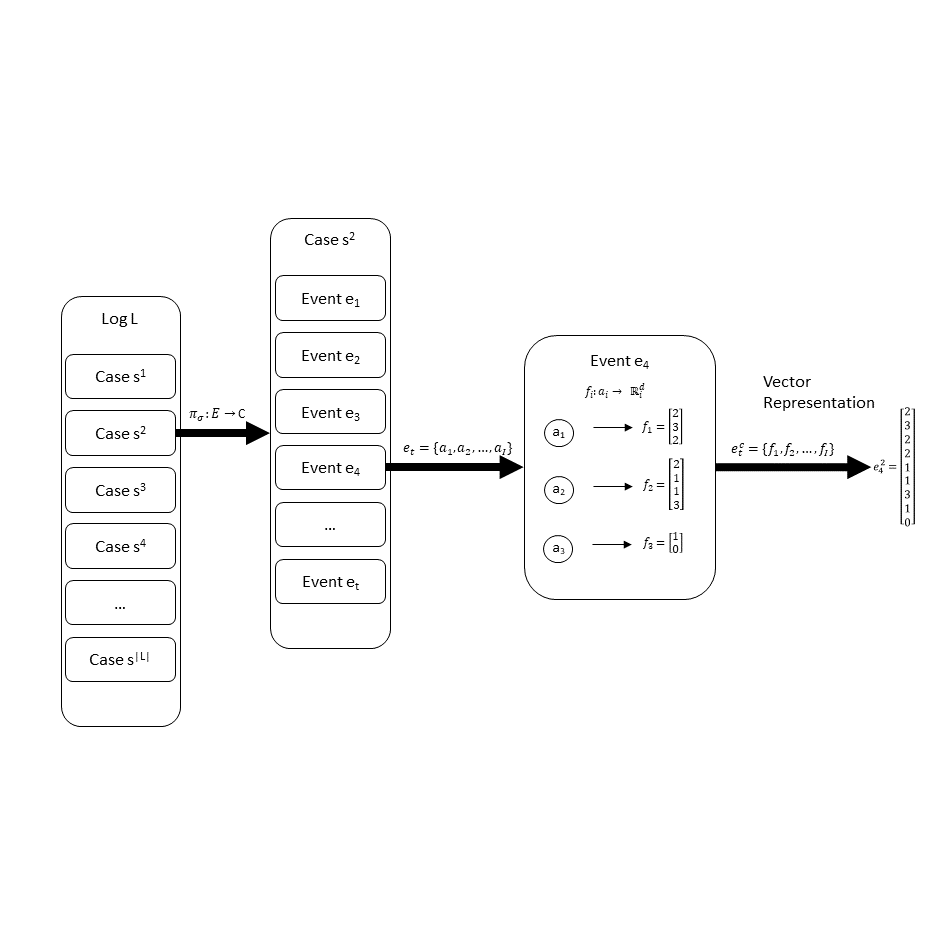
\includegraphics[width=0.9\textwidth]{figures/Graphics/Slide4.PNG}
    \caption{This figure shows the representation of a log $L$ which contains a number of cases $s$. Case $s^2$ contains a number of events $e_t$. Each events has attribute values $a_i$, which are mapped to vector spaces of varying dimensions. At last, all of the vectors are concatenated.}
    \label{fig:representation}
\end{figure}


% , \forall a_i^{\sigma} \in A_i^{\sigma}$
%  A log L is defined as $L =(E, \pi_c, \pi_t, \pi_1 , ..., \pi_{d_n})$
% Each given set of sequences is a case instance $c \in C$ and a surjective function $\pi_\sigma : E \mapsto C$ links every element in $E$ to a case in $C$. 


\subsection{State-Space Models}
% https://en.wikipedia.org/wiki/State-space_representation
Generally speaking, every time-series can be represented as a state-space model\autocite{kalman_NewApproachLinear_1960}. Within this framework the system consists of \emph{input states} for \emph{subsequent states} and \emph{subsequent outputs}. A mathematical form of such a system is shown in \autoref{eq:nonlinear_state_space}.

\begin{align}
    \label{eq:nonlinear_state_space}
    % \begin{gather}
    \nextState & =h(t, \currentState, \currentInput)           \\
    \currentEvent   & =g(t, \currentState, \currentInput) \nonumber \\
    \nextState &:=\frac{d}{d t} \currentState \nonumber
    % \end{gather}
\end{align}

\noindent Here, $\currentInput$ represents the input, $\currentState$ the state at time $t$. The function $h$ maps $t$, $\currentState$ and $\currentInput$ to the next state $\nextState$. The event $\currentEvent$ acts as an output computed by function $g$ which takes the same input as $h$. The variables $\currentState$, $\currentInput$ and $\currentEvent$ are vectors with discrete or continuous features. The distinction of $\nextState$ and $\currentEvent$ decouples \emph{hidden}\footnotemark~states, from \emph{observable} system outputs.
\autoref{fig:nonlinear_state_space} shows a graphical representation of these equations.

\begin{figure}[htb]
    \centering
    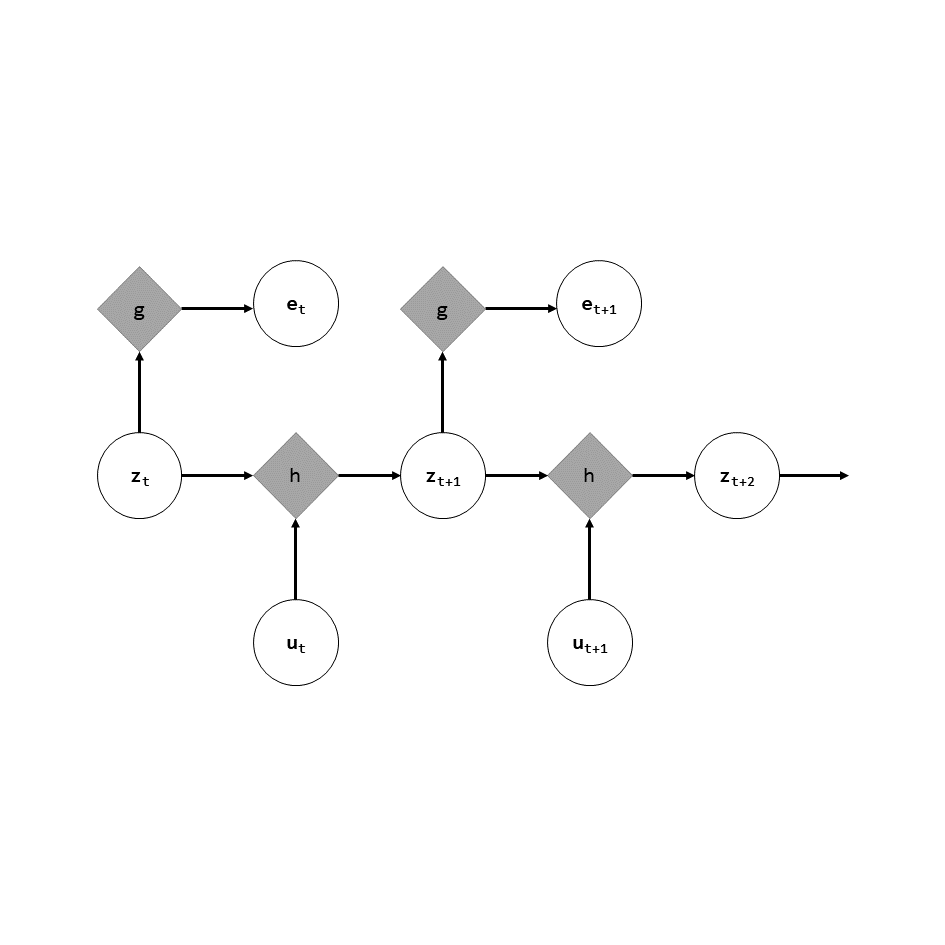
\includegraphics[width=0.9\textwidth]{figures/Graphics/Slide5.PNG}
    \caption{This figure shows a simplified graphical representation of a state-space model. Each arrow represents the flow of information.}
    \label{fig:nonlinear_state_space}
\end{figure}

\footnotetext{A state does not have to be hidden. Especially, if we know the process and the transition rules. However, those are often inaccessible if we only use log data. Instead, many techniques try to approximate the hidden state given the data instead. For an introduction to state-space models see:\autocite{hangos_IntelligentControlSystems_2001}}

The body of literature for state-space models is too vast to discuss them in detail. 
However, for process mining, we can use this representation to discuss the necessary assumptions for process mining.
In line with the process-definition in \autoref{sec:process}, we can understand the \gls{log} as a collection of the observable outputs of a state-space model. 
The state of the process is hidden as the \emph{true} process which generated the data cannot be observed as well. The time $t$ is a step within the process. Hence, we treat $t$ as a discrete scalar value to denote discrete sequential time steps. Hence, if we have $\sigma=\{a,b,b,c\}$, then $t$, describes the index of each element in $\sigma$.  The input $\currentInput$ represents all context information of the process. Here, $\currentInput$ subsumes observable information such as the starting point and \gls{instance}-related features. The functions $h$ and $g$ determine the transition of a process' state to another state and its output over time. Note, that this formulation disregards any effects of future timesteps on the current timestep. Meaning, that the state transitions are causal and therefore, ignorant of the future.
As we establish in \autoref{sec:process}, we can assume that a process is a discrete sequence, whose transitions are time-variant. 
In this framework, we try to identify the parameters of the functions $h$ and $g$. Knowing the functions, it becomes simple to infer viable counterfactuals. However, the function parameters are often unknown and therefore, we require probablistic approaches.

We can formulate \autoref{eq:nonlinear_state_space} probablistically as shown in \autoref{eq:probablistic_state_space}.

\begin{align}
    \label{eq:probablistic_state_space}
    \mathbb{E}[\cProbNextState] & =
    \int z_{t+1} \cdot \cProbNextState \\
    \mathbb{E}[\cProbCurrObservation]   & =
    \int x_{t} \cdot \cProbCurrObservation \nonumber
\end{align}

Note, that $h$ and $g$ are substitued with probability density functions parametrised with $\theta_h$ and $\theta_g$. $T$ signifies the full sequence including future timesteps.
Both expectations are intractable as they require integrating over n-dimensional vectors. To solve the intractability, we characterize the system as a \emph{Hidden Markov Process} and \gls{PGM}. This framework allows us to leverage simplifying assumptions such as the independece from future values and \emph{d-seperation}. 

% The stochastic process is shown in \autoref{fig:prob_state_model}.

% \needsfigure{fig:prob_state_model}{Figure shows a graphical representation of the stochastic process.}

These characteristics change the probabilities in \autoref{eq:probablistic_state_space} to \autoref{eq:encoder_probability}:

\begin{align}
    \label{eq:encoder_probability}
    \cProbNextShortState                   & =  \prod_{1}^{t} \cProbCurrShortState \\
    % \label{eq:decoder_probability}
    \cProbCurrShortObservation                   & = \prod_{1}^{t} \cprob{x_{t-1}}{z_{1:t},\theta_f}
    % \\
    % \label{eq:approx_probablistic_state_space}
    % \hat{z_{t+1}}                & = \mathbb{E}[p(z_{t+1})] \\
    % \hat{x_{t}}                  & = \mathbb{E}[\cprob{x_{t}}{\hat{z_{t}}}] \nonumber
\end{align}

For $\cProbNextState$, we ignore future timesteps, as $T$ changes into $t$. \emph{d-seperation} allows us to ignore all $\currentEvent$ of previous timesteps. The graphical form also decomposes the probability into a product of probabilities that each depend on all previous states and its current inputs. Previous $\currentEvent$ are ignored due to \emph{d-seperation}. $\cProbCurrObservation$ only depends on its current state, which is in line with \glspl{HMM}.
Note, that we deliberately not assume a \emph{strong Markov Property}, as the \gls{DL}-Framework allows us to take all previous states into account. The \emph{strong Markov Property} would assume that only the previous state suffices. At last, we assume that we do not model automatic or any other process whose state changes without a change in the input or previous states. Hence, we remove the dependency on the independent $t$ variable. Only the previous states $z_{1:T}$ and the input information $\currentInput$ remain time-dependent. 

In this probabilistic setting, the generation of counterfactuals, amounts to drawing samples from the likelihood of \autoref{eq:encoder_probability}. We then use the samples to reconstruct the most-likely a counterfactual $e_{1:t}^*$. Hence, our goal is to maximize both likelihoods. 

% TODO: \attention{A number of AI techniques where developed to model this representation bla bla bla (HMM, Kalman, etc -- \href{https://youtu.be/rz76gYgxySo?t=546}{Has further formalisation}).}

\end{document}